\documentclass[12pt,twocolumn]{article}
\usepackage[T1]{fontenc}
\usepackage{graphicx}
\usepackage{tabularx}
\usepackage{amsmath,amsthm,amssymb}
\usepackage[left=1cm,right=1cm,top=2cm,bottom=2cm]{geometry}
%\renewcommand*{\familydefault}{\sfdefault}
\title{\vspace{-2.5em}Convection and Diffusion}
\author{Christopher Pattison}
\date{}
\begin{document}
\maketitle
\section*{Introduction}
The convection diffusion equation \eqref{eq:convdiff} is used to model systems where both diffusion and transport are occurring. 
\begin{equation}\label{eq:convdiff}\nabla\cdot k \nabla T - \nabla\cdot\rho u C_P T -q = 0\end{equation}
\begin{equation}\label{eq:fvmconvdiff}\int_V(\nabla\cdot k \nabla T - \nabla\cdot\rho u C_P T - q)dV = 0\end{equation}
\begin{equation}\label{eq:evalconvdiff}\left. k \frac{dT}{dx} - \rho u C_P T \right\rvert^{x_e}_{x_w}  - qV= 0\end{equation}
After applying the Finite Volume Method in equation \eqref{eq:fvmconvdiff}, equation \eqref{eq:evalconvdiff} is obtained.
\begin{equation}\label{eq:differencesconvdiff}k\frac{T_E-T_P}{x_E-x_P} - k\frac{T_P-T_W}{x_P-x_W}-\rho u C_P T_e + \rho u C_P T_w - qV= 0\end{equation}
Finite Differences are applied giving equation \eqref{eq:differencesconvdiff}.
The interpolation scheme to determine $T_e$ still remains to be selected.

\section*{Convection}
A quantity called the Peclet number can be defined as the ratio of convective flux to diffusive flux \eqref{eq:peclet}.
This is useful for concisely stating how much convection is occurring.
\begin{equation}D = k\Delta x^{-1};\hspace{1ex} F= \rho u C_P\end{equation}
\begin{equation}\label{eq:peclet}P = \frac{F}{D} = \frac{\rho u C_P}{k\Delta x^{-1}}\end{equation}
\subsection*{Central-Differences}
The obvious interpolation scheme for the convective term is a central-difference \eqref{eq:lininter}. However, stability issues can result.
\begin{equation}\label{eq:lininter}T_e = \frac{T_E+T_P}{2} \end{equation}
\begin{equation}\label{eq:lincoeff}a_e = D_e - \frac 12 F_e;\hspace{1ex}a_w = D_w + \frac 12 F_w \end{equation}
As made evident by the formulation of coefficients for a central-difference interpolation \eqref{eq:lincoeff}, a Peclet number above 2 will result in negative coefficients.
\subsection*{Upwinding}
Another option is to take the upwind value of T \eqref{eq:upwind} as the value at the cell face.
\begin{equation}\label{eq:upwind}T_e = \begin{cases}T_P & u>0\\T_E & u\leq 0\end{cases} \end{equation}
While this results in excess diffusion as demonstrated in figure \ref{fig:solution}, it is stable and will give positive coefficients.

\begin{figure}
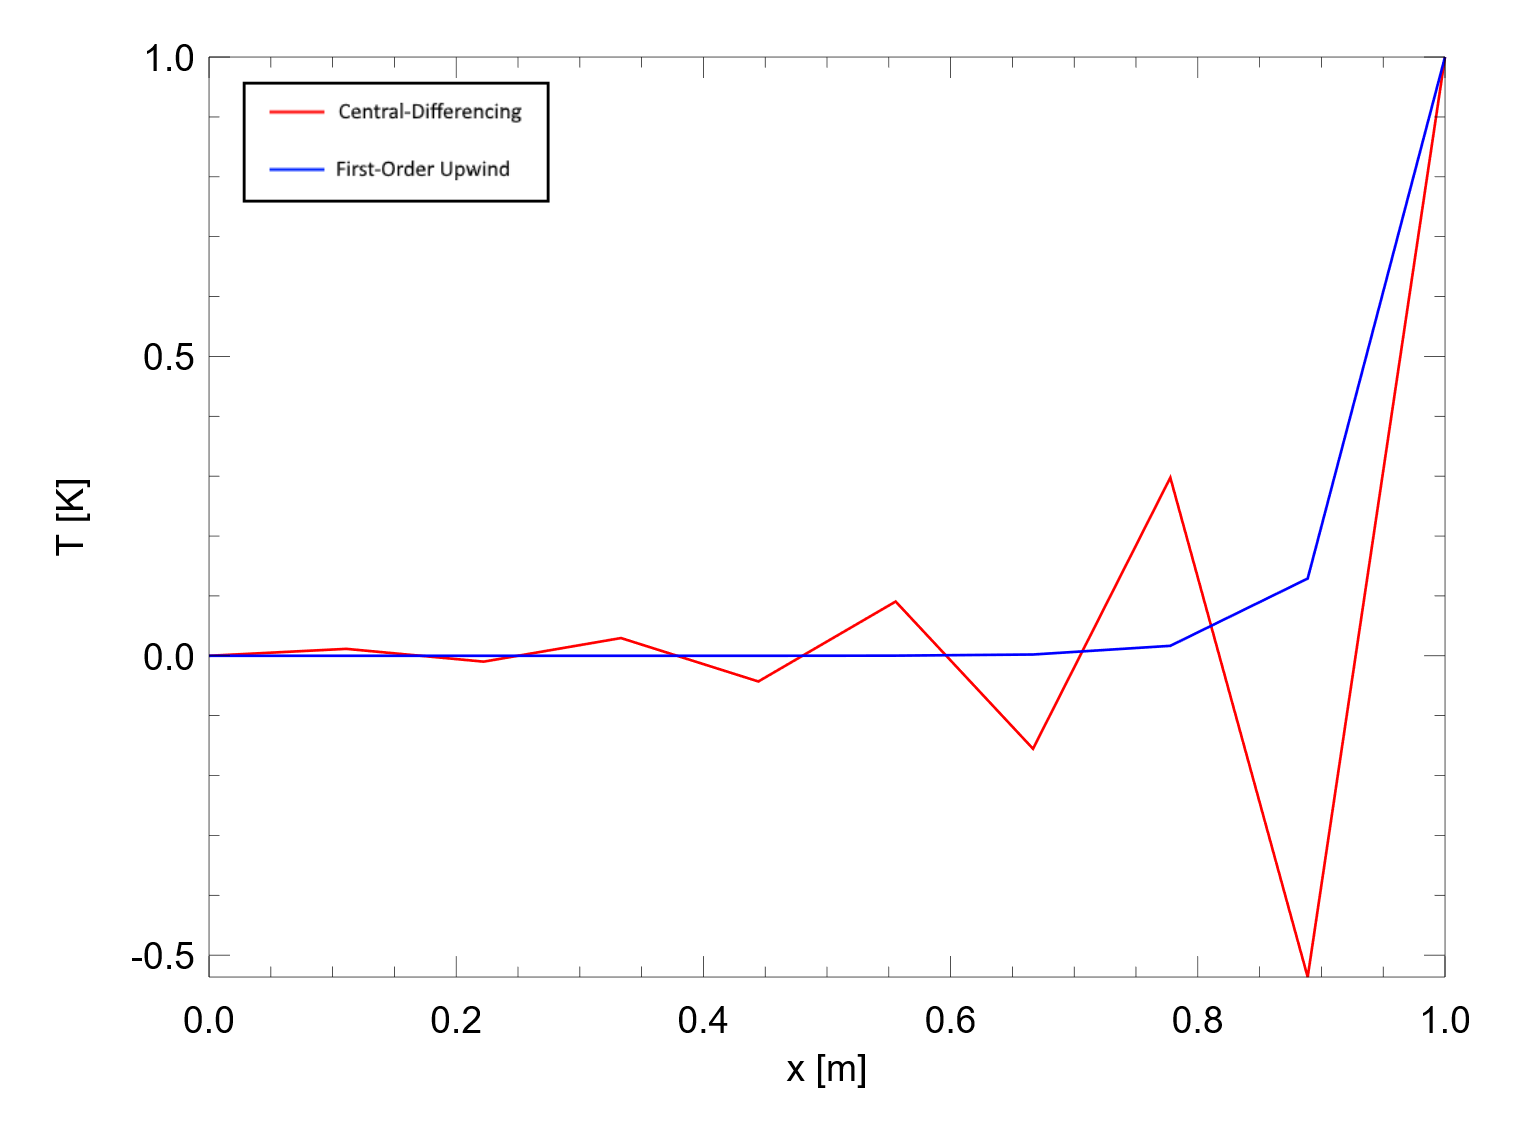
\includegraphics[width=\columnwidth]{plots/solution.png}
\caption{Solution with $P = 50$}
\label{fig:solution}
\end{figure}

\section*{Grid Refinement}
In order for central-differencing to be a viable interpolation scheme, the Peclet number must be reduced.
In the definition of Peclet number \eqref{eq:peclet}, it is evident that $P$ is a function of grid spacing.
Thus, a grid refinement will lower the Peclet number allowing the coefficients to become positive again:
The grid must be refined to use central-differencing.
\subsection*{Selective Refinement}
It is undesirable to refine the entire grid, because of memory and processing constraints.
One approach involves inserting a node into the grid or splitting a cell in two.

\subsection*{Solution}
The grid refinement provided an efficient usage of cells so that central-differencing could be used without instability.
This method would also be useful to refine the grid such that cell size is a function of temperature gradient.

\begin{figure}
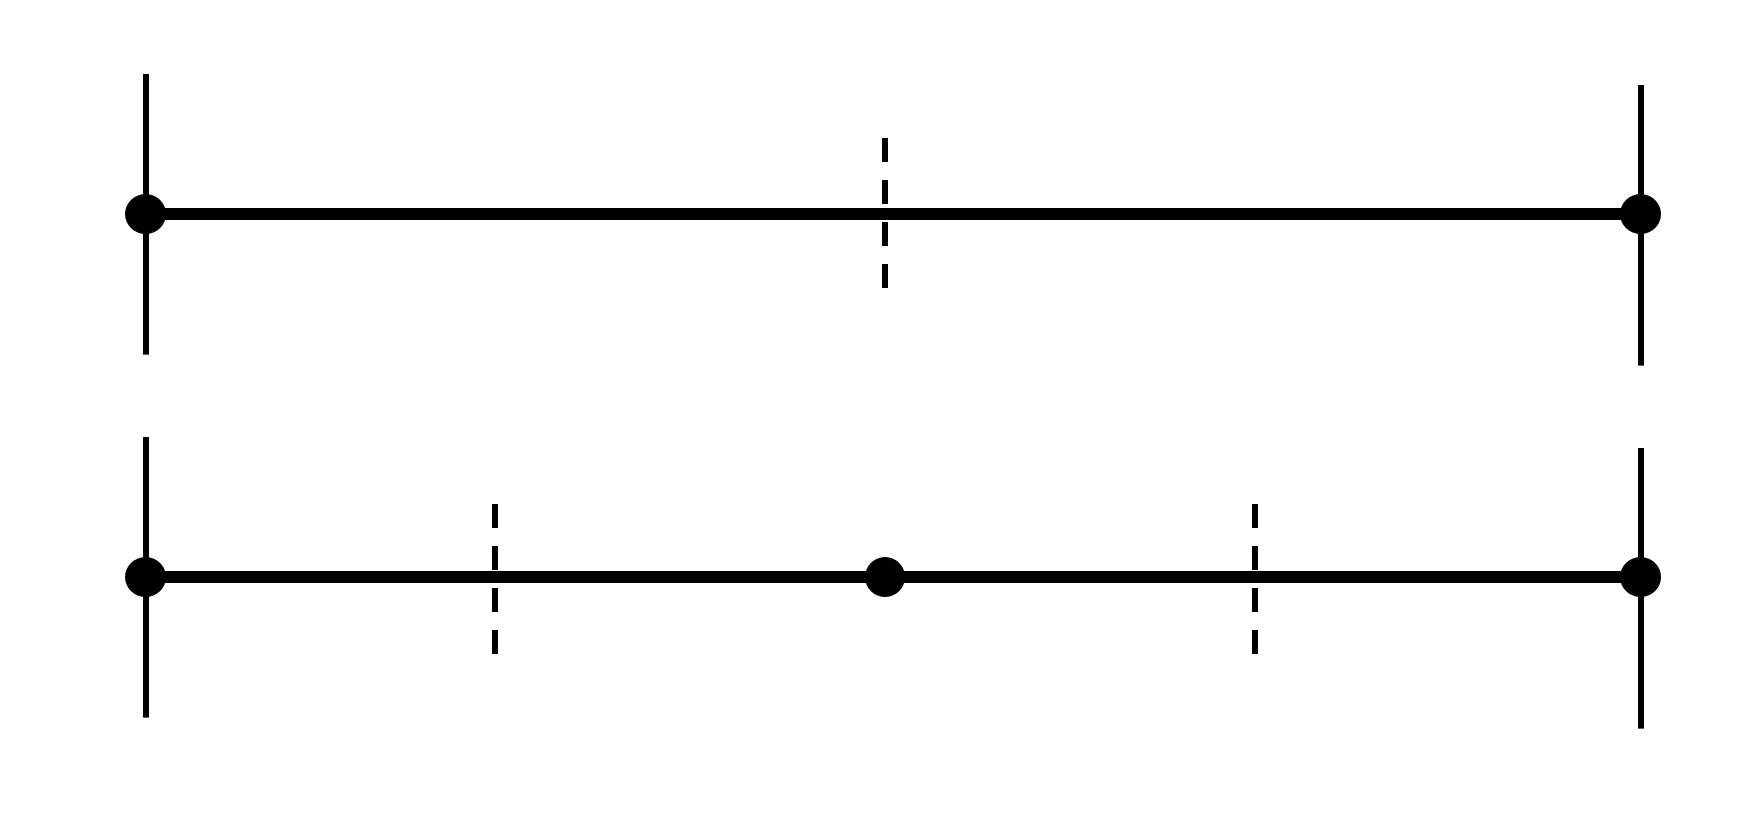
\includegraphics[width=\columnwidth]{plots/cellsplitting.png}
\caption{Cell Splitting}
\label{fig:cellsplitting}
\end{figure}
\end{document}
